\section{Méthode de répartition des données}

\subsection{Motivation et définition de la répartition des données}

Avec l’augmentation continue du volume de données et du nombre d’utilisateurs, les architectures de stockage centralisées atteignent rapidement leurs limites. Une base de données unique n’a plus la capacité de contenir toute ces données et constitue un point de défaillance susceptible de compromettre la disponibilité du système.

\IfFileExists{images/09_central_architecture.png}{
\begin{figure}[!ht]
\centering
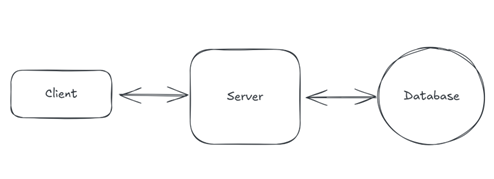
\includegraphics[width=0.7\textwidth]{images/09_central_architecture.png}
\end{figure}
}{}

Une solution pour pallier à ces limitations consiste à répartir les données et les requêtes sur plusieurs bases de données, afin de distribuer la charge de stockage et de traitement, et d’éviter la surcharge d’une base de données unique.

\newpage

\IfFileExists{images/10_distributed_architecture.png}{
\begin{figure}[!ht]
\centering
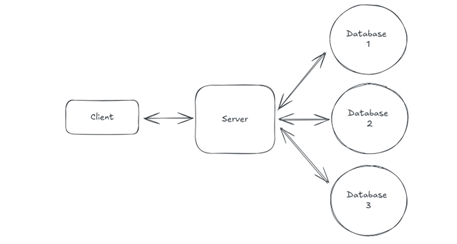
\includegraphics[width=0.7\textwidth]{images/10_distributed_architecture.png}
\end{figure}
}{}

Toutefois, cette distribution soulève un problème fondamental : il devient nécessaire de déterminer de manière systématique sur quelle base de données une donnée doit être stockée et comment la retrouver efficacement. C’est pour répondre à cette problématique que les méthodes de répartition des données (data partitioning ou data sharding) ont été introduites. Elles définissent les règles de placement des données ce qui impacte directement les performances et l’équilibrage de charge. Ces méthodes de répartitions des données impactent également l’évolution du système dans le temps, c’est-à-dire lors de l’ajout ou le retrait d’une base de données.

\subsection{Les différentes méthodes de répartitions des données}

Après avoir montré la nécessité de répartir les données dans un système distribué, la première question qu’on se pose : comment associer chaque donnée à une base de données ?

Différentes méthodes de répartition des données permettent d’associer une clé à une base de données dans un système distribué.

Dans les exemples suivant nous allons utiliser le termes nœud qui fait référence à une instance base de données et le terme évènement qui fait référence à une donnée.

\subsubsection{hachage classique}

\subsubsection*{Principe général du hachage classique}

Une première approche naïve appelée hachage classique (naive hashing ou modulo hashing) consiste à utiliser une fonction de hachage afin de faire la correspondance entre la clé d’une donnée et la base de données dans laquelle nous allons la stocker.

\newpage
\subsubsection*{Association d’une clé à un nœud}

Cette méthode repose sur les étapes suivantes :



\begin{enumerate}
\item Prendre l’id de l’événement et l’exécuter via une fonction de hachage, qui le convertit en nombre
\item Prendre ce nombre et effectuer l’opération modulo (\%) avec le nombre de base de données.
\item Le résultat nous indique quelle base de données doit stocker cet évènement.
\end{enumerate}

La formule serait donc :

\[
\texttt{database\_id} = \texttt{hash(event\_id)} \bmod \texttt{number\_of\_databases}
\]

\IfFileExists{images/11_hash_modulo.png}{
\begin{figure}[!ht]
\centering
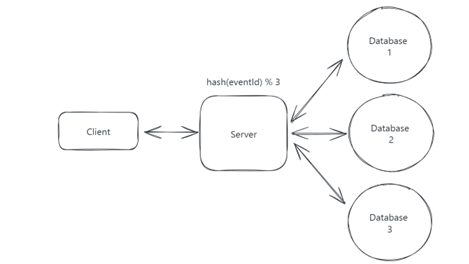
\includegraphics[width=0.6\textwidth]{images/11_hash_modulo.png}
\end{figure}
}{}

Pour un exemple concret avec 3 bases de données :

Event \#1234 → hash(1234) \% 3 = 1 → Database 2

Event \#5678 → hash(5678) \% 3 = 0 → Database 1

Event \#9012 → hash(9012) \% 3 = 2 → Database 3

Ainsi, chaque clé est associée à une base de données unique, ce qui permet de retrouver l’emplacement d’une donnée à partir de sa clé.

\subsubsection*{Limite du hachage classique}

Le premier problème survient lorsque l’on souhaite ajouter une nouvelle instance de base de données. La première solution à laquelle on pourrait penser consisterait à exécuter l'opération modulo avec 4 au lieu de 3 (Par rapport à l’exemple précédent).


database\_id = hash(event\_id) \% 4


La modification du nombre total de bases de données a non seulement affecté les données destinées à la nouvelle instance, mais a également entraîné une modification de la base de données associé à chaque événement précédemment stocké.

En effet, si on reprend un des exemples précédents :

Event \#1234 → hash(1234) \% 3 = 1 → Database 2     hash(1234) \% 4 = 0 → Database 1

L'événement n° 1234 était mappé à la base de données 2, mais avec l’ajout de la nouvelle base de données, ces données doivent donc être déplacées vers la base de données 1.

\newpage
\IfFileExists{images/12_hash_resize_problem.png}{
\begin{figure}[!ht]
\centering
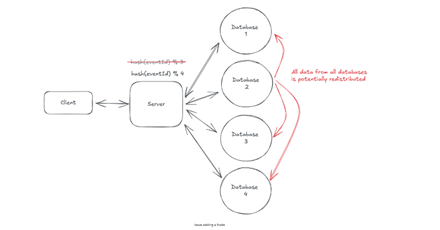
\includegraphics[width=0.7\textwidth]{images/12_hash_resize_problem.png}
\end{figure}
}{}

L’ajout d’une ou plusieurs bases de données entraîne donc une redistribution dans toutes les instances de base de données, ce qui provoque un mouvement massif de données inutiles. Ce mouvement massif cause d'énormes pics de charge de base de données et impact directement les utilisateurs. En effet, les utilisateurs ne pourront pas accéder à leur donner ou auront un temps de réponse lent.


Un autre problème avec le hachage modulo simple réside dans le retrait d’une base de données. Supposons qu'une base de données soit tombée en panne. Il est nécessaire de redistribuer les données qui étaient dans la base de données tombé en panne vers les autres bases de données encore actives. Etant donné que le nombre de base de données actives diminue, le calcule pour trouver où ranger une donnée sera modifié. De ce fait, les données présentes dans les bases de données encore actives risque d’être redistribué vers d’autre instance de base de données.

\IfFileExists{images/13_hash_resize_problem2.png}{
\begin{figure}[!ht]
\centering
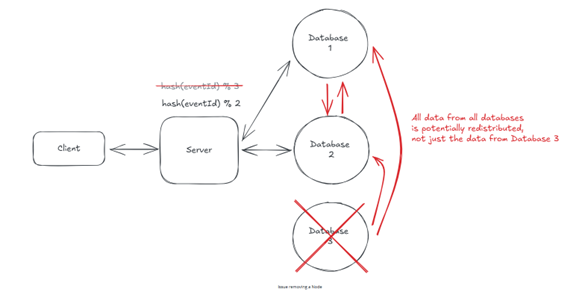
\includegraphics[width=0.7\textwidth]{images/13_hash_resize_problem2.png}
\end{figure}
}{}

Ces limitations montrent que le hachage modulo classique n’est pas adapté aux systèmes distribués dynamiques, où les bases de données peuvent être ajoutés ou retirés fréquemment.

\subsubsection{Hachage cohérent (Consistent Hashing)}

\subsubsection*{Principe général du consistent Hashing}

Le consistent Hashing a été introduit pour résoudre le problème de la redistribution des données lors de l'ajout ou de la suppression d'une instance dans un système distribué. Le principe est d’organiser à la fois les données et les bases de données dans un espace circulaire appelé « anneau de hachage ».

Dans cet anneau, les clés et les nœuds sont positionnés en utilisant la même fonction de hachage. Chaque base de données se voit attribuer une position sur l’anneau, et chaque donnée est également positionnée sur cet anneau en fonction du résultat de sa fonction de hachage.


\subsubsection*{Association d’une clé à un nœud}

Cette méthode repose sur les étapes suivantes :

\begin{enumerate}
\item On réalise d’abord un anneau de hachage avec un nombre fixe de points.
\item On positionne les bases de données sur l’anneau en appliquant la fonction de hachage à leur identifiant.
\item Pour trouver sur quelle base de données une donnée doit être stockée, on hache d'abord l'ID de la donnée comme avec le hachage classique.
\item On se déplace ensuite dans le sens des aiguilles d'une montre sur l’anneau jusqu’à rencontrer le premier nœud.
\item Ce nœud va stocker de la donnée.
\end{enumerate}

Par exemple :

Pour un nombre fixe de points égal à 90, 3 bases de données positionnées aux points 20, 50 et 80.

Si nous avons un $\texttt{hash(id\_data)} = 32$, nous nous déplaçons dans le sens des aiguilles d’une montre pour trouver la première instance de base de données. Cette instance sera la base de données 2 (Node B) située au point 50.

\IfFileExists{images/14_consistent_example.png}{
\begin{figure}[!ht]
\centering
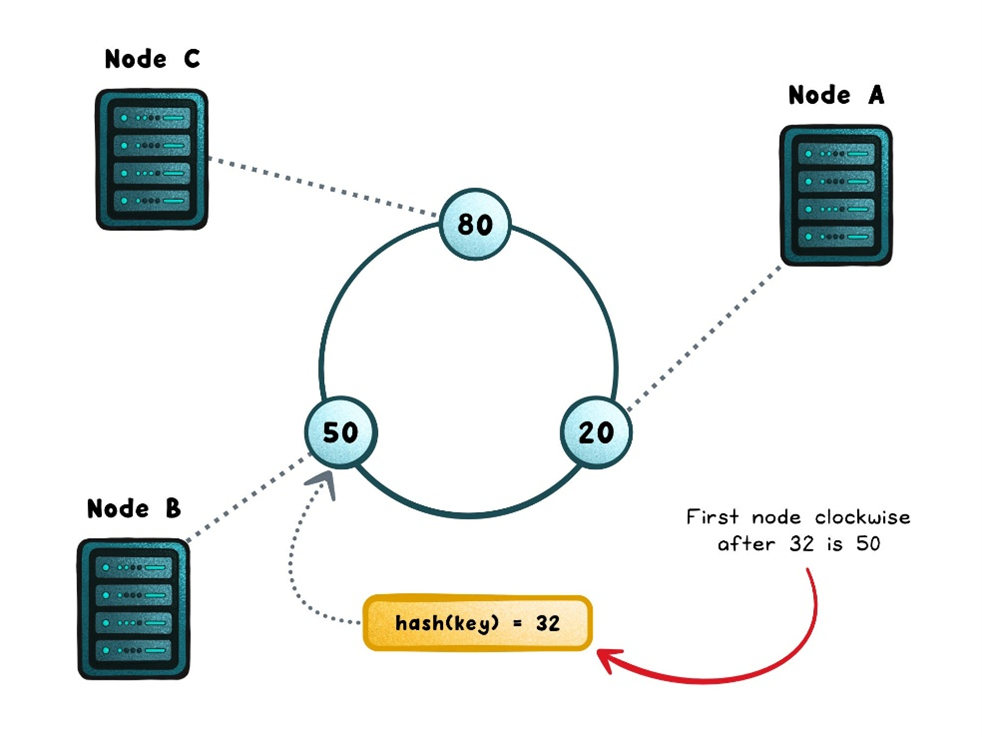
\includegraphics[width=0.75\textwidth]{images/14_consistent_example.png}
\end{figure}
}{}

\subsubsection*{Ajout d’une nouvelle base de données}

Lorsqu’on ajoute une nouvelle base de données, seules les données qui se situent entre sa nouvelle position et la base de données précédente doivent être déplacées.

Par exemple :

Pour un nombre fixe de points égal à 100, 4 bases de données positionnées aux points 0, 25, 50 et 75.

Si nous ajoutons une cinquième base de données à la position 90 sur notre anneau :

\begin{itemize}
	\item Seules les données qui se hachent vers des positions comprises entre 75 et 90 doivent désormais être stockées dans la base de données 5.

  \item Toutes les autres données restent dans leur base de données respective.
\end{itemize}

\IfFileExists{images/15_consistent_add.png}{
\begin{figure}[!ht]
\centering
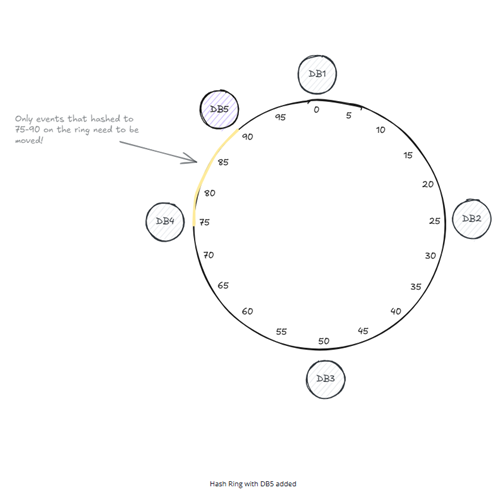
\includegraphics[width=0.75\textwidth]{images/15_consistent_add.png}
\end{figure}
}{}

Contrairement au hachage modulo classique, seule une petite portion des données est redistribuée.

\subsubsection*{Suppression d’une base de données}

En reprenant l’exemple initial :

Pour un nombre fixe de points égal à 100, 4 bases de données positionnées aux points 0, 25, 50 et 75.

Supposons que la base de données numéro 2 située à la position 25 rencontre une défaillance.
\begin{itemize}
  \item Seules les données mappées sur la base de données 2 doivent être déplacées.

  \item Le déplacement se fait dans le sens des aiguilles d’une montre. Elles seront donc mappées à la base de données 3 située à la position 50.

	\item Toutes les autres données restent dans leur base de données respective.
\end{itemize}

\newpage

\IfFileExists{images/16_consistent_remove.png}{
\begin{figure}[!ht]
\centering
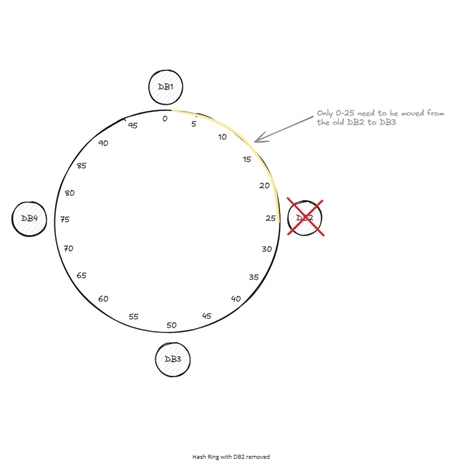
\includegraphics[width=0.75\textwidth]{images/16_consistent_remove.png}
\end{figure}
}{}

Le consistent hashing permet ainsi de résoudre les principales limites du hachage classique en réduisant drastiquement le nombre de données redistribuées lors des changements de topologie (ajout ou retrait de base de données). 

Cependant, il reste encore un problème. En effet, dans notre exemple ci-dessus où nous avons supprimé la base de données 2, nous avons dû déplacer toutes les données stockées dans la base de données 2 vers la base de données 3, ce qui peut entraîner une surcharge locale. Notre objectif serait de répartir de manière équitable les données lors de la suppression d’une base de données.  


\subsubsection*{Optimisation : Nœuds Virtuels}

Pour résoudre ce problème, une des solutions serait d’utiliser des « nœuds virtuels ». Au lieu de mettre chaque base de données en un seul point de sur l’anneau, nous la divisons en plusieurs point en hachant différentes variantes du nom de la base de données. 

Par exemple : 

« DB1 » sera diviser en « DB1-vn1 », « DB1-vn2 », « DB1-vn3 » et « DB1-vn4 » qui seront respectivement aux positions 0, 20, 35, 65, 80. C’est le même principe pour les autres bases de données.

\newpage

\IfFileExists{images/17_virtual_nodes.png}{
\begin{figure}[!ht]
\centering
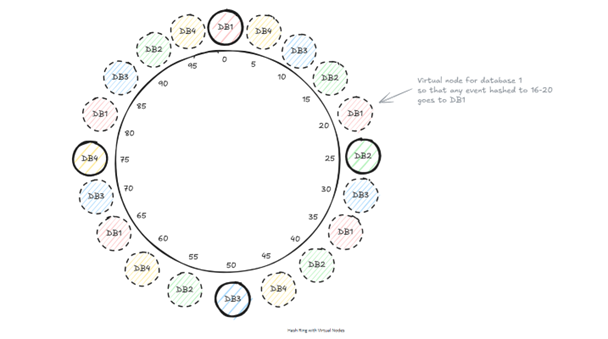
\includegraphics[width=0.8\textwidth]{images/17_virtual_nodes.png}
\end{figure}
}{}

Nous pouvons observer sur la figure ci-dessus que les nœuds virtuelles sont mélangés autour de l’anneau. 
Supposons que la bases de données numéro 2 rencontre une défaillance : 
	
	\begin{itemize}
		\item Les données mappées sur « DB2-vn1 » seront stockées dans la base de données 1
		\item Les données mappées sur « DB2-vn2 » seront stockées dans la base de données 3
    \item Les données mappées sur « DB2-vn3 » seront stockées dans la base de données 4
	  \item Et ainsi de suite
\end{itemize}
La charge de la base de données supprimé est donc répartie de manière beaucoup plus homogène dans toute les bases de données actives. 


\subsection{Conclusion sur les méthodes de répartitions des données}

Les méthodes de répartition des données sont donc indispensables dans les systèmes distribués. En effet, elles déterminent la manière dont les données sont réparties entre les bases de données. Le hachage classique est une solution simple, mais peu adaptée lors de l’ajout ou du retrait d’une ou plusieurs bases de données, en raison des redistributions massives qu’il engendre. Le consistent hashing permet de corriger ces limitations en réduisant les déplacements de données. Une des optimisations du consistent hashing repose sur l’utilisation de nœuds virtuels, permettant d’améliorer l’équilibrage de charge entre les nœuds lors du retrait d’une base de données.
